% =====================================================================
% III. Metodología: construcción del dataset (subsecciones A a G).
% Fragmento sin \section; lo sigue secciones/metodologia_modelos.tex (H a J).
% Niveles de título: \section -> III.  \subsection -> A.  \subsubsection -> 1)
% =====================================================================
\providecommand{\pendiente}[1]{\textcolor{red}{\textbf{[PENDIENTE: #1]}}}
\providecommand{\arch}[1]{\path{#1}}

Esta sección describe, en orden, cómo se pasó del conjunto público original a las 35\,007 imágenes de recortes (ROI) con las que se entrenaron y compararon los cuatro modelos (Secciones~\ref{sec:modelos} y \ref{sec:protocolo}). La Fig.~\ref{fig:flujo} resume el flujo y el número de elementos que pasan por cada etapa. Todas las cifras proceden de los archivos versionados del repositorio.


% ---------------------------------------------------------------------
\subsection{Origen de los datos}
\label{sec:origen}
Se usó el \emph{Lumbar Spine MRI Dataset} (Mendeley Data) \cite{sudirman2019}, que reúne estudios de 515 pacientes con dolor lumbar sintomático y 48\,345 cortes de resonancia magnética, y que ya se ha empleado en trabajos previos sobre clasificación de hernia discal \cite{sari2025} y sobre gradación de la degeneración con la escala de Pfirrmann \cite{natalia2024}. Los estudios se adquirieron con un único equipo, un Siemens MAGNETOM Essenza de 1,5~T, y se distribuyen como archivos DICOM con extensión \arch{.IMA}, en una carpeta por paciente. Las carpetas están numeradas de 0001 a 0575; los 60 números que faltan ya faltan en la fuente. Los cortes tienen un tamaño de píxel de 0,729~mm, un grosor de 4~mm y una separación entre centros de 4,8~mm. Los archivos \texttt{.IMA} conservan sus metadatos DICOM, pero el campo \texttt{PatientID} está vacío en todo el corpus y la fuente solo conserva identificadores de estudio y de serie. Por eso, en este trabajo cada carpeta se trata como un paciente: las 515 carpetas equivalen a los 515 pacientes, y toda mención a ``paciente'', incluida la división por paciente, se refiere a la carpeta.

De los 515 pacientes, 414 conservaron cortes útiles tras la depuración (Sección~\ref{sec:depuracion}) y 399 tras las exclusiones de calidad de los ROI (Sección~\ref{sec:roi}). Cada una de las 414 carpetas corresponde a un \texttt{StudyInstanceUID} distinto y no se repite ningún \texttt{StudyTime}; no hay evidencia de pacientes duplicados, aunque con el identificador vacío no puede descartarse del todo.

\begin{figure}[!htb]
\centering
\begin{tikzpicture}[
  box/.style={draw, rounded corners=2pt, align=left, text width=0.56\columnwidth, inner sep=2pt, font=\scriptsize},
  num/.style={align=left, text width=0.34\columnwidth, font=\scriptsize\bfseries},
  arrow/.style={-{Stealth[length=1.5mm]}, thick},
  node distance=3mm]
  \node[box] (a) {1. Conjunto público (Mendeley), archivos \texttt{.IMA}};
  \node[num, right=2mm of a] {515 pacientes, 48\,345 cortes};
  \node[box, below=of a] (b) {2. Filtrado por nombre de serie (T2 sagital)};
  \node[num, right=2mm of b] {8\,794 cortes};
  \node[box, below=of b] (c) {3. 40\,\% central, DICOM$\to$PNG y limpieza manual};
  \node[num, right=2mm of c] {1\,086 cortes, 414 pacientes};
  \node[box, below=of c] (d) {4. Recorte L1--S1 y detección de discos (ROI 128$\times$128)};
  \node[num, right=2mm of d] {5\,385 ROI};
  \node[box, below=of d] (e) {5. Preetiquetado, revisión humana y exclusiones};
  \node[num, right=2mm of e] {5\,123 ROI, 399 pacientes};
  \node[box, below=of e] (f) {6. División por paciente 70/15/15};
  \node[num, right=2mm of f] {279 / 60 / 60 pacientes};
  \node[box, below=of f] (g) {7. Aumento dentro de cada partición};
  \node[num, right=2mm of g] {35\,007 imágenes};
  \foreach \i/\j in {a/b,b/c,c/d,d/e,e/f,f/g} \draw[arrow] (\i) -- (\j);
\end{tikzpicture}
\caption{Flujo de preparación del dataset y número de elementos en cada etapa.}
\label{fig:flujo}
\end{figure}

% ---------------------------------------------------------------------
\subsection{Depuración de la fuente}
\label{sec:depuracion}
Cada paciente trae varias series y solo una parte sirve para este problema. La Tabla~\ref{tab:descartes} lista lo que se descartó y por qué.

\begin{table}[!htb]
\centering\footnotesize
\caption{Series descartadas de cada estudio y motivo}
\label{tab:descartes}
\begin{tabular}{>{\raggedright\arraybackslash}p{0.33\columnwidth}>{\raggedright\arraybackslash}p{0.58\columnwidth}}
\toprule
Serie & Motivo del descarte \\
\midrule
\arch{LOCALIZER_0001} & Localizadores de muy baja resolución para posicionar al paciente; no aportan información anatómica ni de textura. \\
\arch{POSDISP_[4]_T2_TSE_TRA_...} & Vistas sagitales con líneas superpuestas (\emph{overlays}) que marcan los planos transversales y distorsionan la textura. \\
\arch{T1_TSE_SAG_...}, \arch{T1_TSE_TRA_...} & En T1 la grasa es brillante y el líquido oscuro: no permite evaluar la hidratación del disco, base de la escala de Pfirrmann \cite{pfirrmann2001}, y mezclar T1 y T2 altera los rangos de brillo. \\
\arch{T2_TSE_TRA_...} (axial) & Cortes axiales en lotes de 3 a 5 por nivel; exigirían emparejarlos con cada disco. Se deja para una fase futura. \\
\arch{T2_TIRM_SAG_...} & Inversión-recuperación con supresión grasa, de contraste distinto al T2 TSE. Se eliminó en la depuración manual. \\
\bottomrule
\end{tabular}
\end{table}

El proceso se hizo en cuatro pasos, cada uno con su script (carpeta \arch{scripts/preprocesamiento/}); la Tabla~\ref{tab:etapas} da el número de cortes y de pacientes tras cada uno.
\begin{enumerate}
  \item \arch{ingestion.py} copia los archivos cuyo nombre contiene ``T2'' y ``SAG'', salvo localizadores y \arch{POSDISP}. Ese criterio dejó pasar, además de la serie T2 TSE sagital, la serie T2 TIRM sagital de 44 pacientes.
  \item \arch{limpiar_slices.py} conserva el 40\,\% central de los cortes de cada paciente (descarta el 30\,\% inicial y el 30\,\% final, ordenados por nombre de archivo), donde el canal medular y la región L1--S1 son visibles.
  \item \arch{convertidor_dcm_a_png.py} convierte a PNG de 8 bits con una sola escala por serie: percentiles 1 y 99,5 calculados sobre los píxeles de tejido. No se aplicó CLAHE ni otro realce, para no alterar la señal relativa del T2 que sustenta el criterio diagnóstico; la forma de normalizar la intensidad influye en el desempeño del aprendizaje profundo en resonancia, al menos en segmentación \cite{jimenezpartinen2026}, por lo que se mantuvo una sola normalización, por serie, en todo el corpus.
  \item Depuración manual de los PNG: se eliminaron los estudios del segmento cervical o de rodillas, los cortes T2 sagitales oscuros o con aberraciones, y todos los cortes TIRM.
\end{enumerate}

\begin{table}[!htb]
\centering\footnotesize
\caption{Cortes (por secuencia) y pacientes tras cada paso de la depuración}
\label{tab:etapas}
\begin{tabular}{lrrrr}
\toprule
Paso & TSE & TIRM & Total & Pacientes \\
\midrule
Corpus original & -- & -- & 48\,345 & 515 \\
Filtrado por nombre & 8\,094 & 700 & 8\,794 & 515 \\
40\,\% central & 3\,235 & 284 & 3\,519 & 515 \\
Depuración manual & 1\,086 & 0 & 1\,086 & 414 \\
\bottomrule
\end{tabular}
\end{table}

Tras esta depuración quedaron \textbf{1\,086 cortes sagitales T2 TSE de 414 pacientes} (2,6 cortes por paciente en promedio; entre 1 y 6).

\subsubsection{Error en la selección de cortes}
Al revisar la trazabilidad, una vez construido el dataset, se encontró un error en el paso~2. En los 44 pacientes que tenían serie TIRM, el 40\,\% central se calculó sobre la lista conjunta de ambas series ordenada por nombre. Como los archivos TIRM se ordenan antes que los TSE, la ventana conservada abarcó los cortes centrales del TIRM y los primeros cortes del TSE (del 1 al 6 de 15), que son laterales. En la depuración manual se eliminaron los TIRM y, en 36 de esos 44 pacientes, no quedó ningún corte TSE útil: son 36 de los 101 pacientes que se pierden entre 515 y 414. Los otros 8 entraron con el corte 006 de 15, parasagital y no medio-sagital. Ningún corte TIRM llegó al dataset final. Filtrar solo la serie \arch{T2_TSE_SAG} y elegir el corte medio-sagital dentro de esa serie, como hacen otros trabajos sobre este mismo corpus \cite{natalia2024}, habría conservado esos pacientes. Por falta de tiempo no se rehizo el proceso y el error se declara como limitación. Además, 17 pacientes tienen 30 cortes TSE (posiblemente dos series) y podrían estar afectados por el mismo cálculo; no se verificó.

% ---------------------------------------------------------------------
\subsection{Recorte de la región lumbar y de los ROI por disco}
\label{sec:roi}
\subsubsection{Recorte L1--S1}
Con \arch{aplicar_recortes.py} se recortó cada corte en altura para abarcar principalmente L1--S1, replicando por \emph{template matching} unos recortes manuales previos (mediana de la puntuación de coincidencia 0,9996; solo el corte 0547\_008 quedó por debajo de 0,99). El recorte se extendió 60~px hacia arriba y hacia abajo hasta el borde de la imagen; con ello el relleno necesario en L1-L2 bajó de 779 de 1\,080 recortes (72\,\%) a cero.

\subsubsection{Detector de discos}
Detectar los discos antes de clasificarlos es un paso habitual en la literatura, incluida la familia YOLO sobre cortes sagitales \cite{tan2024,sayed2025scirep}. Para localizarlos se entrenó un detector con un conjunto propio en Roboflow (proyecto \emph{Intervertebral Disks}, versión~1): 100 cortes (70 de entrenamiento, 20 de validación y 10 de prueba), con orientación automática y reescalado a 640$\times$640 con bordes negros, sin aumento de datos en Roboflow. Las cinco clases del detector son los niveles L1-L2 a L5-S1. Se ajustó un YOLOv8n de detección de cajas. El modelo que generó los ROI se entrenó durante 100 épocas; una versión de 200 épocas se descartó porque, al inspeccionar sus detecciones, marcaba discos donde no los había. El detector solo ubica el nivel del disco; no clasifica patología.

Aunque Roboflow no aplicó aumento, Ultralytics aplica por defecto un aumento en línea durante el entrenamiento (mosaico, escala, traslación, variación de color y reflexión horizontal con probabilidad 0,5). La reflexión no cambia el nivel de un disco, porque el orden de L1-L2 a L5-S1 es vertical; en el aumento del dataset de clasificación, en cambio, se excluyó (Sección~\ref{sec:aumento}).

El cuaderno con el que se entrenó el modelo usado no guardó sus métricas. Para reportar el desempeño se repitió el entrenamiento con los mismos datos y la misma arquitectura (50 épocas, paciencia 30, lote 16, imagen de 640~px, semilla 42 y el mismo aumento por defecto; mejor época en validación: 49). La Tabla~\ref{tab:detector} resume esa repetición con el umbral de uso (confianza 0,35).

\begin{table*}[t]
\centering\footnotesize
\caption{Desempeño de la repetición del entrenamiento del detector (corrida \texttt{detector\_discos\_v1\_s42}), usada como estimación del modelo que generó los ROI}
\label{tab:detector}
\begin{tabular}{lrrrrrrr}
\toprule
Partición & Cortes & Precisión & Recall & mAP50 & mAP50-95 & Cortes con 5 niveles & IoU medio \\
\midrule
Validación & 20 & 0,922 & 0,964 & 0,962 & 0,663 & 95\,\% & 0,819 \\
Prueba     & 10 & 0,983 & 0,994 & 0,995 & 0,691 & 100\,\% & 0,843 \\
\bottomrule
\end{tabular}
\end{table*}

El nivel más difícil es L1-L2 (en validación: precisión 0,839, recall 0,820 e IoU 0,74); los demás tienen recall de 1,0. Con solo 20 y 10 cortes, un corte mueve varios puntos porcentuales; es una sola corrida con una sola semilla, y la época se eligió con la validación, por lo que sus cifras están algo infladas. Además, describen la repetición y no el modelo usado, aunque ambos comparten datos y arquitectura y difieren en el número de épocas.

\subsubsection{Extracción del ROI}
Con \arch{autocrop_rois.py} se detecta sobre el recorte y se extrae el parche sobre el PNG completo, sumando el desplazamiento. La caja se amplía (margen posterior 0,40, anterior 0,10 y vertical 0,50), se hace cuadrada y se guarda a 128$\times$128~px, una por nivel. Cada recorte queda registrado en \arch{roi_log.csv} con su caja, su ordenada central, su confianza y el relleno por lado. El resultado fueron \textbf{5\,385 ROI}. El margen anterior de L5-S1 se probó en 0,20 frente a 0,10 y la ganancia fue marginal, por lo que se mantuvo 0,10. La Fig.~\ref{fig:rois} muestra los cinco ROI de un corte.

\begin{figure*}[t]
\centering
\includegraphics[width=0.85\textwidth]{rois_0188_008.png}
\caption{Los cinco ROI originales (L1-L2 a L5-S1) del corte 008 del paciente 0188, tal como quedan en el dataset (128$\times$128~px).}
\label{fig:rois}
\end{figure*}

\subsubsection{Exclusiones por calidad}
Se aplicaron reglas objetivas sobre \arch{roi_log.csv} (función \arch{elegibles()} de \arch{scripts/build_dataset.py}): se descarta el corte completo si falta algún nivel, si dos niveles adyacentes se solapan (IoU $>0{,}5$) o si el orden vertical de los centros no crece de L1-L2 a L5-S1; además se excluyen el paciente 0456, el corte 0547\_008 y los ROI con confianza del detector menor que 0,5. En total se excluyeron \textbf{262 ROI}, que afectan a 48 pacientes; 15 pacientes quedaron fuera por completo. Así, los 5\,385 ROI etiquetados quedan en \textbf{5\,123 ROI de 399 pacientes}. De los ROI excluidos, 207 eran Protrusión, 38 Normal y 17 Degeneración.

% ---------------------------------------------------------------------
\subsection{Anotación y retiquetado}
\label{sec:anotacion}
\subsubsection{Clases}
La guía de anotación (\arch{docs/guias/guia_anotacion_4_clases.md}) define cuatro clases nominales: Normal, Degeneración, Abombamiento y Hernia. Degeneración se definió como pérdida de señal T2 del disco o de su altura sin protrusión, en la línea de la escala de Pfirrmann \cite{pfirrmann2001}. Cuando coinciden varias clases, se aplica la prioridad Hernia $>$ Abombamiento $>$ Degeneración $>$ Normal, que solo sirve para desempatar el etiquetado y no es un orden de gravedad. La guía recoge criterios de uso común y no está validada por un radiólogo. Las etiquetas las asignaron estudiantes, sin radiólogo.

\subsubsection{Fusión a tres clases}
En la primera corrida del clasificador semilla, con las cuatro clases (60 imágenes de validación), la exactitud fue 0,65 (IC 95\,\%: 0,52--0,76) y 10 de los 21 errores fueron confusiones Hernia--Abombamiento. Sin un corte axial, la extensión del abultamiento sobre la circunferencia del disco, que es lo que separa ambas entidades en la nomenclatura de consenso \cite{fardon2014}, no puede medirse. Incluso con una nomenclatura estandarizada, la concordancia entre radiólogos sobre el contorno discal es solo de aceptable a moderada \cite{arana2011}, y en tomografía computarizada se ha reportado que abultamiento y protrusión son el par de clases más confundido \cite{gao2025}. Por eso Hernia y Abombamiento se fusionaron en \textbf{Protrusión}, quedando tres clases: Normal, Degeneración discal y Protrusión. La fusión es una decisión posterior a ver los datos (\emph{post hoc}) y se declara así.

\subsubsection{Preetiquetado y revisión}
Etiquetar 5\,385 ROI desde cero no era viable en el plazo, así que se siguió un esquema de preetiquetado con revisión humana, emparentado con el aprendizaje activo \cite{wang2024al} y con la anotación iterativa en la que un modelo propone y una persona corrige \cite{vandergraaf2024}. Primero se etiquetó a mano en Roboflow una semilla balanceada de unos 300 ROI con las cuatro clases originales: 240 de entrenamiento (60 por clase) y 60 de validación (15 por clase). Roboflow reescaló las imágenes a 224$\times$224 y generó tres salidas por imagen de entrenamiento (rotación de $\pm 5^{\circ}$ y brillo de $\pm 15\,\%$). Las etiquetas se refinaron en tres versiones, a medida que se afinaban los criterios morfológicos y se pasaba a tres clases; en la última se retiraron algunas imágenes. La versión~3, usada para el preetiquetado, tiene 719 imágenes de entrenamiento (ya aumentadas) y 84 de validación (24 Degeneración, 30 Normal y 30 Protrusión). Con ella se entrenó un clasificador pequeño, YOLOv8s-cls (entrada 224$\times$224, hasta 60 épocas, paciencia 15, lote 32, semilla 42). En validación alcanzó una exactitud de 0,833 (IC 95\,\%: 0,739--0,898) y un F1 de 0,784 en Degeneración, 0,852 en Normal y 0,857 en Protrusión; con solo 84 imágenes de validación estas cifras son una guía y no una garantía. El preetiquetador fue una herramienta interna: no es ninguno de los cuatro modelos comparados y su única función fue acelerar y ordenar la revisión.

El modelo preetiquetó los 5\,385 ROI con su clase y su confianza (media 0,946; mediana 1,0) y marcó 2\,265 (42,1\,\%) para revisión prioritaria. Las predicciones de Protrusión se enviaron siempre a revisión (2\,039, de las cuales 1\,881 solo por ese motivo), porque la muestra inicial de 70 ROI sugería que era minoritaria y se esperaba que el modelo, entrenado con clases equilibradas, la sobrepredijera. Las otras 226 se marcaron por confianza menor que 0,7, solo o junto con un margen menor que 0,2 entre las dos primeras clases. La revisión mostró lo contrario: el modelo subestimó la Protrusión.

Después, todos los ROI, marcados o no, pasaron por revisión humana en dos grupos, A y B, de 2\,693 y 2\,692 ROI respectivamente. La clase final es siempre la decisión humana. De los 5\,385 ROI, 3\,366 (62,5\,\%) conservaron la clase del modelo y \textbf{2\,019 (37,5\,\%) fueron corregidos}. La Tabla~\ref{tab:reetiquetado} muestra cómo se reorganizó el dataset.

\begin{table}[!htb]
\centering\footnotesize
\setlength{\tabcolsep}{3.5pt}
\caption{Clase propuesta por el preetiquetador frente a la clase final tras la revisión humana (5\,385 ROI)}
\label{tab:reetiquetado}
\begin{tabular}{lrrrrr}
\toprule
 & \multicolumn{3}{c}{Clase final} & & \\
\cmidrule(lr){2-4}
Predicha & Normal & Degen. & Protr. & Total & Corregidas \\
\midrule
Normal       & 1\,086 & 32  & 1\,387 & 2\,505 & 56,6\,\% \\
Degeneración & 51     & 256 & 534    & 841    & 69,6\,\% \\
Protrusión   & 6      & 9   & 2\,024 & 2\,039 & 0,7\,\% \\
\midrule
Total final  & 1\,143 & 297 & 3\,945 & 5\,385 & 37,5\,\% \\
\bottomrule
\end{tabular}
\end{table}

De los 3\,945 ROI de Protrusión finales, 1\,921 (48,7\,\%) llegaron como Normal o Degeneración, mientras que casi nada de lo que el modelo predijo como Protrusión cambió (15 de 2\,039). La revisión humana, y no el modelo, fijó la distribución de clases del dataset, y esa distribución está muy desbalanceada (Sección~\ref{sec:balance}).

\subsubsection{Fiabilidad de las etiquetas}
Cada ROI fue revisado por una sola persona (A o B); 408 de los 414 pacientes tienen ROI revisados por ambos, pero no hay ROI doble. En consecuencia \textbf{no puede calcularse el coeficiente kappa entre anotadores}. Sí se observan diferencias de criterio: A etiquetó Degeneración en el 6,9\,\% de sus ROI y B en el 4,1\,\%, y corrigió el 35,3\,\% frente al 39,7\,\% de B. No es posible separar cuánto de esa diferencia es criterio y cuánto es composición de la muestra. Las etiquetas de no expertos introducen ruido que reduce la capacidad de generalizar de las redes \cite{shi2024}. Además, como los revisores veían la sugerencia del modelo, cabe un sesgo de anclaje: en radiología se ha observado que un consejo incorrecto de una IA arrastra el diagnóstico de los médicos \cite{prinster2024}.

% ---------------------------------------------------------------------
\subsection{División por paciente}
\label{sec:split}
Cada paciente aporta unos 13 ROI (5\,123/399) de cortes vecinos casi idénticos. Si se dividiera por imagen, un paciente quedaría repartido entre entrenamiento y prueba y el modelo podría reconocer al paciente en lugar de la patología, inflando las métricas (fuga de datos) \cite{brunekreef2024,rumala2023}. Por eso \textbf{cada paciente va entero a una sola partición}.

El reparto es 70/15/15 por pacientes, con semilla 42. El script prueba 20\,000 repartos aleatorios y conserva el que mejor mantiene, en las tres particiones, la proporción de cada clase (con peso triple) y de cada nivel. Se eligieron tres particiones porque la validación sirve para decidir (época, hiperparámetros, umbrales) y la prueba para medir una sola vez al final, con todo ya decidido. La Tabla~\ref{tab:split} muestra el resultado. La intersección de pacientes entre particiones es vacía y se comprueba con aserciones en el script. Los pacientes con al menos un ROI de Degeneración son 81, 17 y 22 en entrenamiento, validación y prueba.

\begin{table}[!htb]
\centering\footnotesize
\setlength{\tabcolsep}{3.5pt}
\caption{División por paciente y ROI originales por clase}
\label{tab:split}
\begin{tabular}{lrrrrrr}
\toprule
Partición & Pacientes & Normal & Degen. & Protr. & ROI & \% ROI \\
\midrule
Entrenamiento & 279 & 771   & 194 & 2\,612 & 3\,577 & 69,8 \\
Validación    & 60  & 170   & 44  & 564    & 778    & 15,2 \\
Prueba        & 60  & 164   & 42  & 562    & 768    & 15,0 \\
\midrule
Total         & 399 & 1\,105 & 280 & 3\,738 & 5\,123 & 100 \\
\bottomrule
\end{tabular}
\end{table}

% ---------------------------------------------------------------------
\subsection{Aumento de datos}
\label{sec:aumento}
Para disponer de más de 35\,000 imágenes con la misma cantidad por clase en cada partición, a partir de 5\,123 ROI originales, se recurrió a aumento de datos. El aumento se hizo siempre \emph{después} de dividir y \emph{dentro} de cada partición, para que ninguna copia cruce de partición: remuestrear antes de dividir sesga al alza las métricas \cite{demircioglu2024}. La cantidad de copias por ROI se calcula para que cada clase alcance la misma meta por partición: 8\,167 imágenes por clase en entrenamiento y 1\,751 en validación y en prueba, es decir 35\,007 en total (Tabla~\ref{tab:35k} y Fig.~\ref{fig:balance}).

\begin{table*}[t]
\centering\footnotesize
\caption{Imágenes finales por partición y clase (mismo número por clase en cada partición), ROI originales e imágenes por original}
\label{tab:35k}
\begin{tabular}{llrrrr}
\toprule
Partición & Clase & Originales & Aumentadas & Total & Imágenes por original \\
\midrule
Entrenamiento & Normal       & 771    & 7\,396 & 8\,167 & 10,6 \\
              & Degeneración & 194    & 7\,973 & 8\,167 & 42,1 \\
              & Protrusión   & 2\,612 & 5\,555 & 8\,167 & 3,1  \\
Validación    & Normal       & 170    & 1\,581 & 1\,751 & 10,3 \\
              & Degeneración & 44     & 1\,707 & 1\,751 & 39,8 \\
              & Protrusión   & 564    & 1\,187 & 1\,751 & 3,1  \\
Prueba        & Normal       & 164    & 1\,587 & 1\,751 & 10,7 \\
              & Degeneración & 42     & 1\,709 & 1\,751 & 41,7 \\
              & Protrusión   & 562    & 1\,189 & 1\,751 & 3,1  \\
\midrule
Total         &              & 5\,123 & 29\,884 & 35\,007 & \\
\bottomrule
\end{tabular}
\end{table*}

\subsubsection{Transformaciones}
Se usaron transformaciones geométricas y fotométricas leves, habituales en imagen médica \cite{islam2024}: rotación de $\pm 8^{\circ}$, desplazamiento de hasta $\pm 8\,\%$ del tamaño, zoom entre 0,90 y 1,10, y brillo y contraste de $\pm 10\,\%$, con reflejo en los bordes. No se usan reflexiones (el eje anterior--posterior tiene significado anatómico), deformación elástica ni realce. Cada copia se genera con una semilla derivada de un hash (SHA-256) del nombre del ROI, la semilla global y el índice de la copia, por lo que el proceso es determinista y reproducible.

\begin{figure}[!htb]
\centering
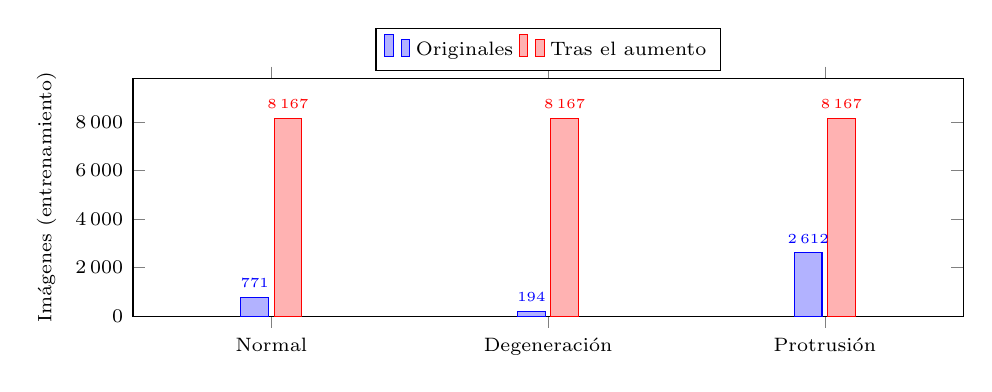
\begin{tikzpicture}
\begin{axis}[
  ybar, bar width=10pt, width=\columnwidth, height=4.6cm,
  symbolic x coords={Normal,Degeneración,Protrusión}, xtick=data,
  ymin=0, ymax=9800, ylabel={Imágenes (entrenamiento)},
  enlarge x limits=0.25, legend style={at={(0.5,1.03)},anchor=south,legend columns=2,font=\scriptsize},
  nodes near coords, every node near coord/.append style={font=\tiny, /pgf/number format/.cd,1000 sep={\,}},
  tick label style={font=\scriptsize}, ylabel style={font=\scriptsize},
  yticklabel style={/pgf/number format/.cd,1000 sep={\,}}, scaled y ticks=false]
\addplot coordinates {(Normal,771) (Degeneración,194) (Protrusión,2612)};
\addplot coordinates {(Normal,8167) (Degeneración,8167) (Protrusión,8167)};
\legend{Originales, Tras el aumento}
\end{axis}
\end{tikzpicture}
\caption{Balance por conteo en entrenamiento: ROI originales y total tras el aumento.}
\label{fig:balance}
\end{figure}

\subsubsection{Trazabilidad}
Cada archivo se llama \arch{T2_TSE_SAG__0188_008_L4-L5__orig.png} (original) o \arch{..._aug012.png} (copia), con paciente, corte y nivel. El manifiesto \arch{manifest_35k.csv} registra, para cada una de las 35\,007 imágenes, su partición, clase, paciente, nivel, ROI original, revisor y, en las copias, los parámetros exactos (semilla, ángulo, zoom, desplazamientos, contraste y brillo); \arch{split_pacientes.csv} guarda la partición de cada paciente. Las imágenes no se suben al repositorio: se distribuyen como un archivo comprimido de 405~MB, y el repositorio guarda los manifiestos y los scripts que las reproducen a partir de los datos públicos.

\subsubsection{Verificaciones}
El script comprueba que (i) los conjuntos de pacientes de las tres particiones son disjuntos, (ii) toda copia está en la misma partición que su original, (iii) los nombres de archivo son únicos, (iv) todo PNG está íntegro y (v) el total supera los 35\,000. Las copias respetan los rangos declarados (ángulo entre $-8^{\circ}$ y $8^{\circ}$, zoom y contraste entre 0,90 y 1,10).

% ---------------------------------------------------------------------
\subsection{Balance de clases y sesgo por nivel}
\label{sec:balance}
El balance de 1/3 por clase es \emph{por conteo}, no por originales. Entre los 5\,123 ROI originales, la Protrusión es el 73,0\,\% (3\,738), Normal el 21,6\,\% (1\,105) y Degeneración el 5,5\,\% (280); un clasificador que siempre dijera Protrusión acertaría cerca del 73\,\%. Las copias igualan la contribución de cada clase al entrenamiento, pero no añaden anatomía nueva: el tamaño efectivo del dataset es el número de pacientes (399), y la Degeneración, repetida unas 42 veces, solo tiene 42 originales en la partición de prueba, lo que deja un margen de error amplio en su recall. Para que las métricas no se inflen con copias casi idénticas, los resultados principales se calculan sobre los \textbf{originales} de la partición de prueba, y el conjunto completo se reporta aparte. Además, un modelo entrenado con prior uniforme tiende a sobrepredecir las clases raras en la población real.

La Tabla~\ref{tab:nivel} muestra un sesgo importante: casi toda la patología se concentra en L4-L5 y L5-S1. Un clasificador que solo adivinara la clase más frecuente de cada nivel acertaría 3\,842 de 5\,123 ROI (75,0\,\%), de modo que el nivel podría actuar como atajo; el aprendizaje por atajos hace que el desempeño medido sobreestime el real \cite{onglt2024}. Por ello los resultados se reportan también por nivel. Esto relativiza cualquier umbral de exactitud: un 95\,\% medido sobre estas etiquetas mide acuerdo con etiquetas de estudiantes y puede alcanzarse en parte por el atajo, y cifras internas altas suelen bajar al evaluar con datos externos \cite{yi2023}. Por eso se acompaña la exactitud con F1 macro y recall por clase: con clases desbalanceadas, las métricas habituales quedan dominadas por la clase mayoritaria \cite{mosquera2024}.

\begin{table}[!htb]
\centering\footnotesize
\setlength{\tabcolsep}{4pt}
\caption{ROI originales elegibles por nivel y clase}
\label{tab:nivel}
\begin{tabular}{lrrrrr}
\toprule
Nivel & Normal & Degen. & Protr. & Total & \% Protr. \\
\midrule
L1-L2 & 505 & 121 & 401    & 1\,027 & 39,0 \\
L2-L3 & 383 & 94  & 550    & 1\,027 & 53,6 \\
L3-L4 & 172 & 44  & 811    & 1\,027 & 79,0 \\
L4-L5 & 15  & 5   & 1\,005 & 1\,025 & 98,0 \\
L5-S1 & 30  & 16  & 971    & 1\,017 & 95,5 \\
\bottomrule
\end{tabular}
\end{table}
